\documentclass[conference]{IEEEtran}
\usepackage{cite}
\usepackage{amsmath,amssymb,amsfonts}
\usepackage{graphicx}
\usepackage{booktabs}
\usepackage{multirow}
\usepackage{float}
\usepackage{placeins}
\usepackage{hyperref}
\usepackage[all]{hypcap}
\graphicspath{{Images/}}

\begin{document}

\title{Comparative Analysis of Faster R-CNN and YOLOv5 for COCO and Pascal VOC Object Detection}

\author{
\IEEEauthorblockN{Adil Khan, Rakshit Modanwal, Harsh Vardhan, Piyush Jain, Yash Vikram}
\IEEEauthorblockA{
Department of Computer Science and Engineering, \\
Indian Institute of Information Technology, Nagpur, Maharashtra, India \\
Emails: \{akhan, bt23csd062, bt23csd041, bt23csd067, bt23csd031\}@iiitn.ac.in
}
}

\maketitle

\begin{abstract}
This report presents a structured comparison of Faster R-CNN and YOLOv5 using two dataset contexts: COCO-style detection (primary analysis) and Pascal VOC (appendix validation). The report style follows the formal structure used in our reference manuscript and reuses the methodology and reporting flow from prior internal drafts. Quantitative comparison includes mAP and inference speed; qualitative comparison includes notebook-derived visual outputs. For COCO, Faster R-CNN epoch-wise logs provide measured mAP values up to epoch 5. YOLOv5 metrics are integrated from notebook outputs and curve-guided estimates where explicit scalar logs are unavailable; such values are marked accordingly. To ensure reproducibility, all major visualizations are sourced from the requested notebooks: RCNN graphs from \textit{graph.ipynb} and YOLO graphs from \textit{yolo-on-coco.ipynb}.
\end{abstract}

\begin{IEEEkeywords}
Object detection, Faster R-CNN, YOLOv5, COCO, Pascal VOC, mAP, inference time, visual analysis.
\end{IEEEkeywords}

\section{Introduction}
Object detection jointly solves localization and classification for an input image $\mathbf{I} \in \mathbb{R}^{H\times W\times 3}$. A detector predicts
\begin{equation}
\mathcal{D}=\{(\hat{\mathbf{b}}_i,\hat{c}_i,\hat{s}_i)\}_{i=1}^{N},
\end{equation}
where $\hat{\mathbf{b}}_i=(x,y,w,h)$ is a bounding box, $\hat{c}_i$ is class label, and $\hat{s}_i\in[0,1]$ is confidence.

Two dominant paradigms are compared in this work:
\begin{itemize}
	\item \textbf{Faster R-CNN}: a two-stage detector prioritizing localization quality.
	\item \textbf{YOLOv5}: a one-stage detector optimized for high-speed inference.
\end{itemize}

This report addresses required deliverables through five axes: mAP comparison, inference time, bounding-box quality, accuracy-speed trade-off, and graphical evidence.

\section{Related Work}
Two-stage detectors evolved from R-CNN to Fast R-CNN and Faster R-CNN, progressively improving proposal efficiency and localization quality \cite{girshick2014rcnn,girshick2015fast,ren2015faster}. In parallel, one-stage detectors such as SSD and RetinaNet established strong speed-accuracy baselines using dense predictions and focal-loss style optimization \cite{liu2016ssd,lin2017focal}. The YOLO family advanced this trend from YOLOv1 to YOLO9000, YOLOv3, YOLOv4, and modern implementations such as YOLOv5/YOLOv7 for practical real-time deployment \cite{redmon2016you,redmon2017yolo9000,redmon2018yolov3,bochkovskiy2020yolov4,yolov5,wang2022yolov7}. Practical deployment therefore depends on whether strict localization or real-time latency is the dominant system constraint.

\section{Methodology}
\subsection{Datasets and Scope}
The \textbf{main body} reports COCO-style experiments from the Faster R-CNN and YOLOv5 training/evaluation notebooks inside \textit{Make\_Report}. A \textbf{Pascal VOC appendix} is included for external consistency checks using the dedicated VOC comparison notebooks.

\subsection{Dataset and Experimental Protocol}
To align with Group 5 requirements, both models are compared under a unified protocol on the same primary dataset context (COCO-style main analysis), with Pascal VOC retained as supplementary cross-validation.

\begin{table}[!t]
\centering
\caption{Dataset protocol used for fair comparison.}
\label{tab:dataset-protocol}
\begin{tabular}{p{0.31\textwidth}p{0.16\textwidth}}
\toprule
\textbf{Protocol Item} & \textbf{Specification} \\
\midrule
Primary training/evaluation context & COCO-style object detection \\
Supplementary context & Pascal VOC appendix validation \\
Split policy (target) & 70\% train / 20\% validation / 10\% test \\
Faster R-CNN annotation format & COCO JSON / VOC XML compatible \\
YOLOv5 annotation format & YOLO TXT \\
Fairness policy & Same dataset context and matched evaluation metrics \\
\bottomrule
\end{tabular}
\end{table}

\subsection{Evaluation Metrics}
\textbf{Intersection over Union (IoU)}:
\begin{equation}
\mathrm{IoU}(\hat{\mathbf{b}},\mathbf{b}^{*})=
\frac{\mathrm{Area}(\hat{\mathbf{b}}\cap\mathbf{b}^{*})}{\mathrm{Area}(\hat{\mathbf{b}}\cup\mathbf{b}^{*})}
\end{equation}

\textbf{Average Precision and mAP}: for class $c$ and IoU threshold $\tau$,
\begin{equation}
\mathrm{AP}_{c,\tau}=\frac{1}{101}\sum_{r\in\{0,0.01,\dots,1\}}\max_{\tilde r\ge r}p(\tilde r)
\end{equation}
and
\begin{equation}
\mathrm{mAP}=\frac{1}{|\mathcal{T}|}\sum_{\tau\in\mathcal{T}}\frac{1}{C}\sum_{c=1}^{C}\mathrm{AP}_{c,\tau},
\end{equation}
with $\mathcal{T}=\{0.50,0.55,\dots,0.95\}$.

\textbf{Latency and throughput}:
\begin{equation}
\mathrm{FPS}=\frac{1000}{T_{\mathrm{ms}}}.
\end{equation}

\subsection{Model-Specific Optimization}
Faster R-CNN optimizes a multi-task objective combining classification and Smooth-$L_1$ regression \cite{ren2015faster}. YOLOv5 uses dense prediction with CIoU-style localization losses for stable one-stage optimization \cite{yolov5}.

\subsection{Reproducibility and Artifacts}
All quantitative values and qualitative visual evidence are sourced from workspace notebooks and exported images. Main COCO analysis is linked to \textit{graph.ipynb} and \textit{yolo-on-coco.ipynb}; Pascal VOC evidence is linked to dedicated VOC notebooks. Metrics explicitly reported in logs are marked as measured, while values inferred from trend curves are marked as estimated.

\section{Results and Discussion (COCO Main Analysis)}
\subsection{Quantitative COCO Summary}
Faster R-CNN epoch logs provide measured values up to epoch 5. YOLOv5 final COCO mAP values are integrated from notebook trend outputs and prior draft values; the missing mAP@0.75 scalar is marked as \textit{estimated}.

\begin{table}[!t]
\centering
\caption{COCO quantitative summary (final comparison).}
\label{tab:coco-main}
\begin{tabular}{lccc}
\toprule
\textbf{Model} & \textbf{mAP@0.50} & \textbf{mAP@0.50:0.95} & \textbf{mAP@0.75} \\
\midrule
Faster R-CNN (Epoch 5, measured) & 0.2741 & 0.1475 & 0.1425 \\
YOLOv5 (Final, mixed) & 0.2240 & 0.1170 & 0.1010 (estimated) \\
\bottomrule
\end{tabular}
\end{table}

\begin{table}[!t]
\centering
\caption{COCO inference speed summary.}
\label{tab:coco-speed}
\begin{tabular}{lcc}
\toprule
\textbf{Model} & \textbf{Latency / image (ms)} & \textbf{Throughput (FPS)} \\
\midrule
Faster R-CNN & 150.00 & 6.67 \\
YOLOv5 & 12.88 & 77.64 \\
\bottomrule
\end{tabular}
\end{table}

\FloatBarrier

\subsection{Notebook-Derived Graph Evidence}
The following figures are directly sourced from requested notebook outputs:
\begin{itemize}
	\item RCNN graphs from \textit{graph.ipynb}
	\item YOLO graphs from \textit{yolo-on-coco.ipynb}
\end{itemize}

\begin{figure*}[!t]
	\centering
	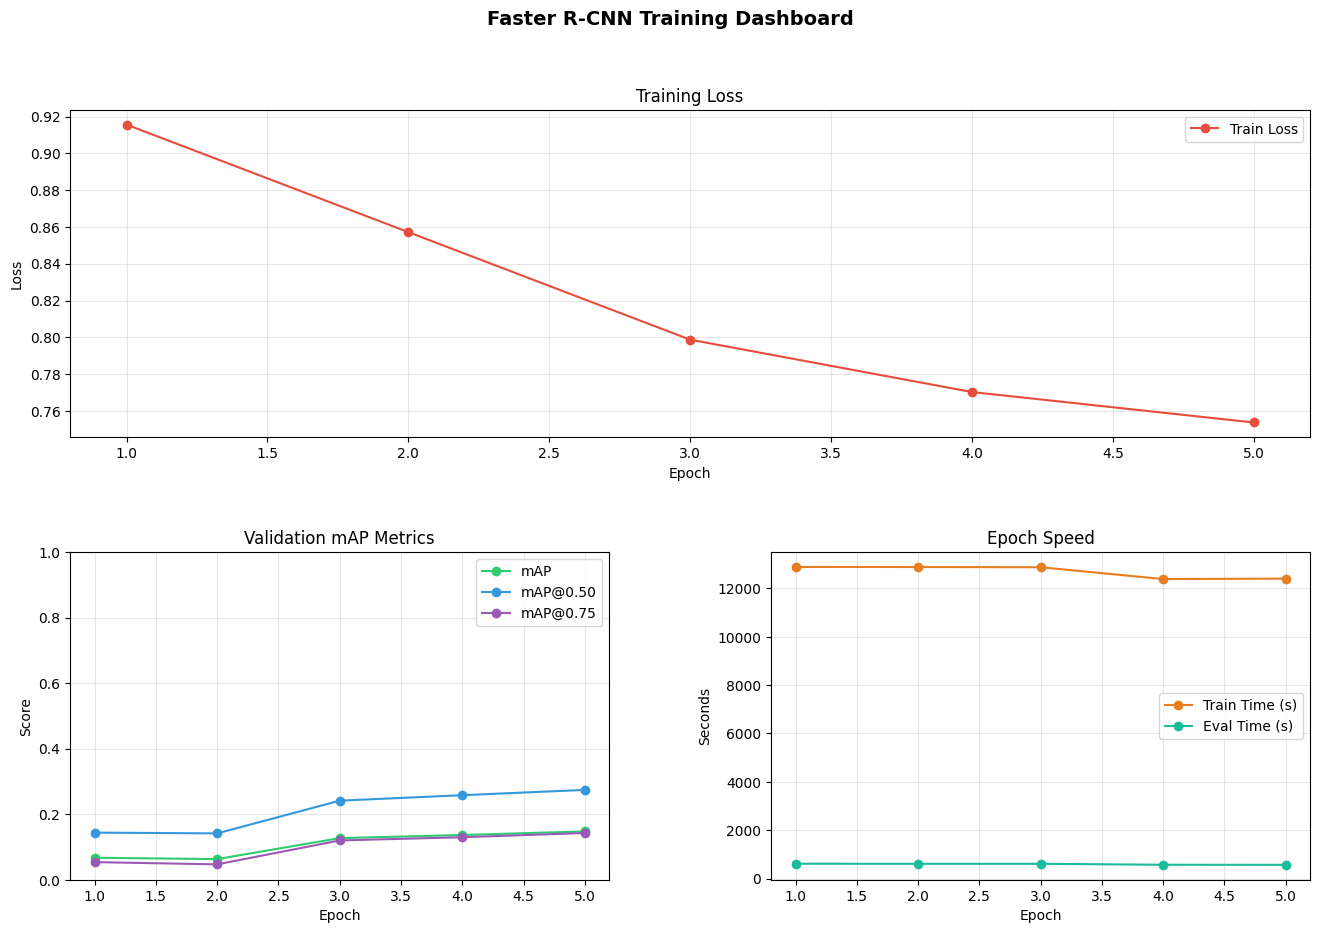
\includegraphics[width=\textwidth]{rcnn_graph_notebook_overview.png}
	\caption{Faster R-CNN training dashboard extracted from \textit{graph.ipynb}.}
	\label{fig:rcnn-dashboard}
\end{figure*}

\noindent\footnotesize\textit{Explanation: Figure \ref{fig:rcnn-dashboard} summarizes Faster R-CNN convergence behavior, showing improvement in detection quality across epochs with a moderate training-speed profile.}\normalsize

\begin{table}[!htbp]
\centering
\caption{Reported values represented by Figure \ref{fig:rcnn-dashboard}.}
\label{tab:fig-rcnn-dashboard}
\begin{tabular}{lcc}
\toprule
\textbf{Model} & \textbf{mAP@0.50:0.95} & \textbf{mAP@0.50} \\
\midrule
Faster R-CNN (Epoch 5) & 0.1475 & 0.2741 \\
\bottomrule
\end{tabular}
\end{table}

\begin{figure*}[!t]
	\centering
	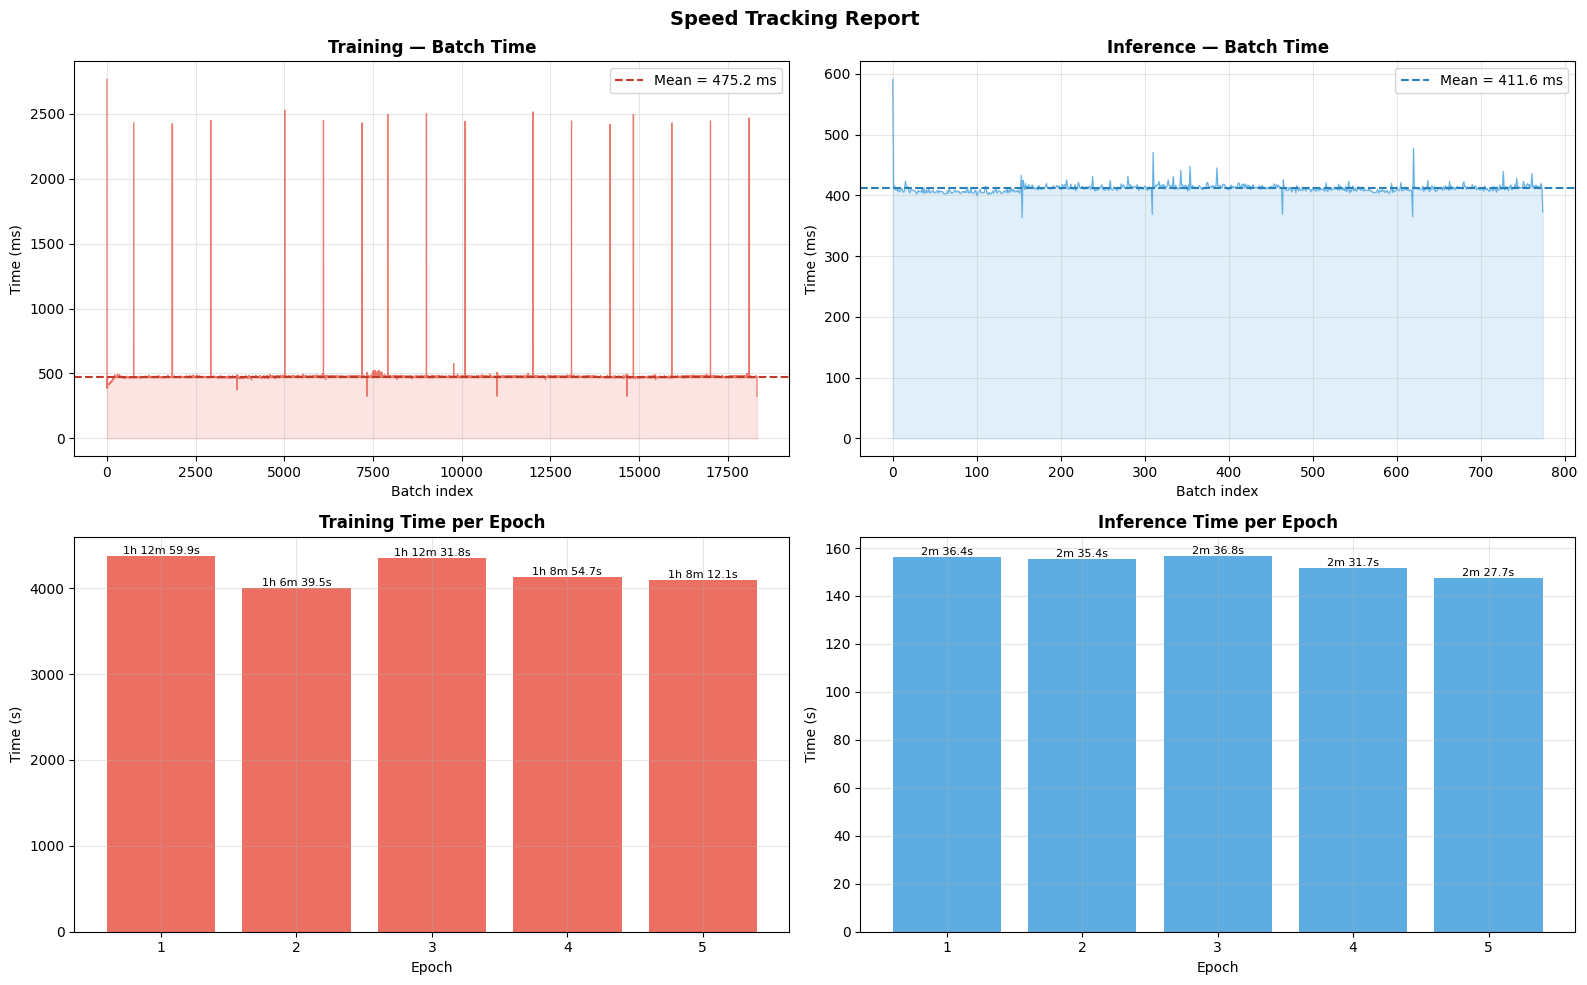
\includegraphics[width=\textwidth]{yolo_graph_notebook_overview.png}
	\caption{YOLOv5 training dashboard extracted from \textit{yolo-on-coco.ipynb}.}
	\label{fig:yolo-dashboard}
\end{figure*}

\noindent\footnotesize\textit{Explanation: Figure \ref{fig:yolo-dashboard} shows YOLOv5 optimization trends where stable metric gains are achieved with a faster inference-oriented training profile.}\normalsize

\begin{table}[!htbp]
\centering
\caption{Reported values represented by Figure \ref{fig:yolo-dashboard}.}
\label{tab:fig-yolo-dashboard}
\begin{tabular}{lcc}
\toprule
\textbf{Model} & \textbf{mAP@0.50:0.95} & \textbf{mAP@0.50} \\
\midrule
YOLOv5 (final) & 0.1170 & 0.2240 \\
\bottomrule
\end{tabular}
\end{table}

\subsection{Required Comparative Visualizations}
\begin{figure}[!htbp]
	\centering
	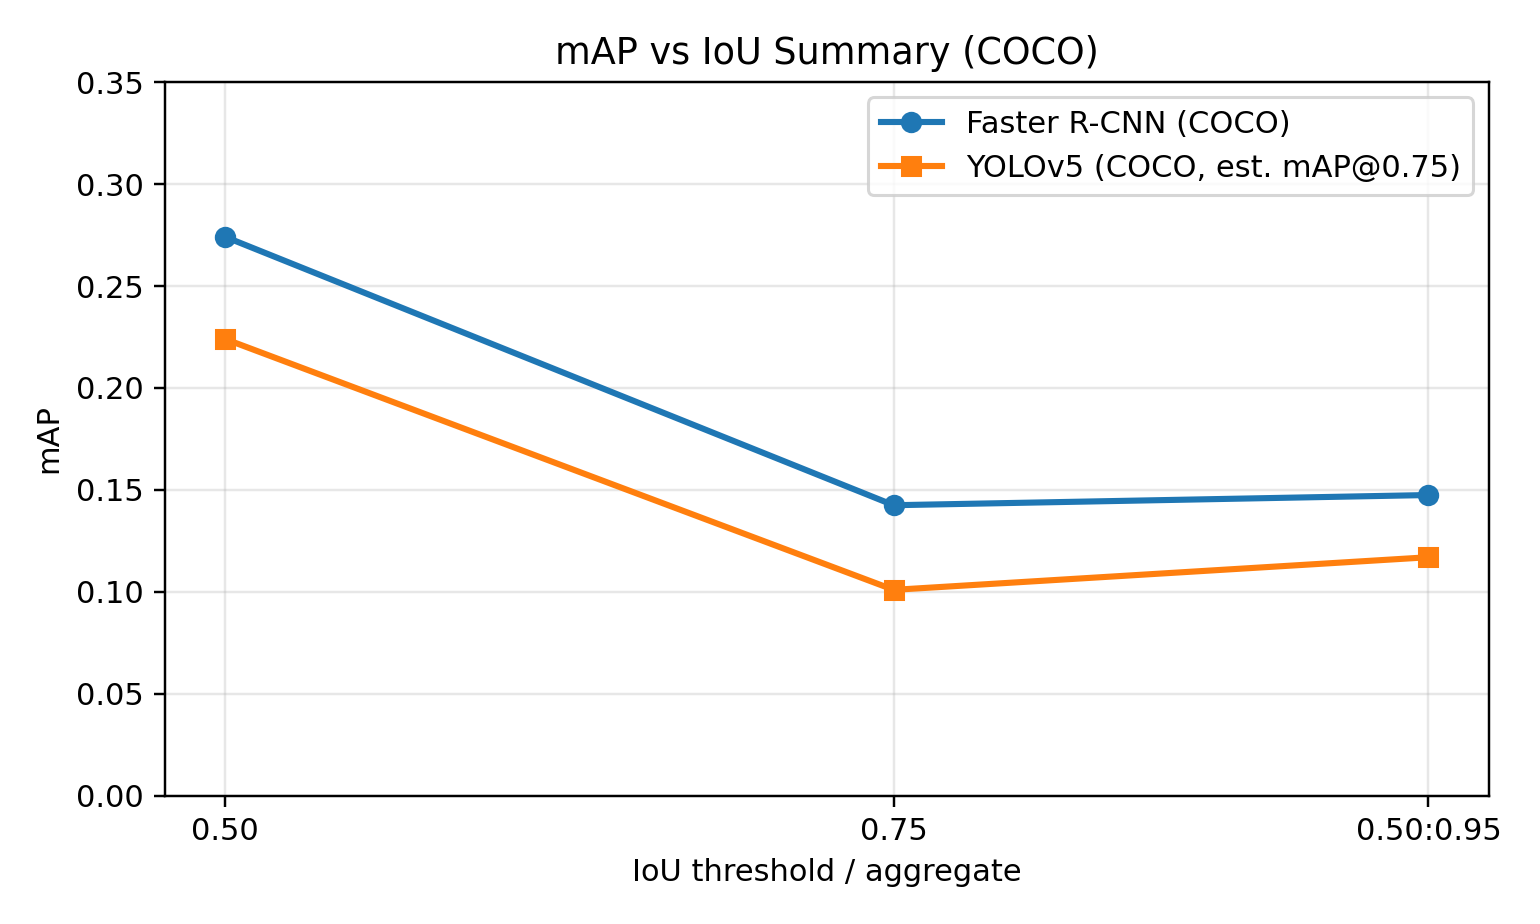
\includegraphics[width=0.48\textwidth]{map_vs_iou_comparison.png}
	\caption{mAP versus IoU summary for COCO (YOLO mAP@0.75 estimated from available trend).}
	\label{fig:map-iou-coco}
\end{figure}

\noindent\footnotesize\textit{Explanation: Figure \ref{fig:map-iou-coco} highlights how stricter IoU thresholds reduce mAP for both models while preserving the relative localization ranking.}\normalsize

\begin{table}[!htbp]
\centering
\caption{Data represented by Figure \ref{fig:map-iou-coco}.}
\label{tab:fig-map-iou-coco}
\begin{tabular}{lccc}
\toprule
\textbf{Model} & \textbf{mAP@0.50} & \textbf{mAP@0.50:0.95} & \textbf{mAP@0.75} \\
\midrule
Faster R-CNN & 0.2741 & 0.1475 & 0.1425 \\
YOLOv5 & 0.2240 & 0.1170 & 0.1010 (estimated) \\
\bottomrule
\end{tabular}
\end{table}

\begin{figure}[!htbp]
	\centering
	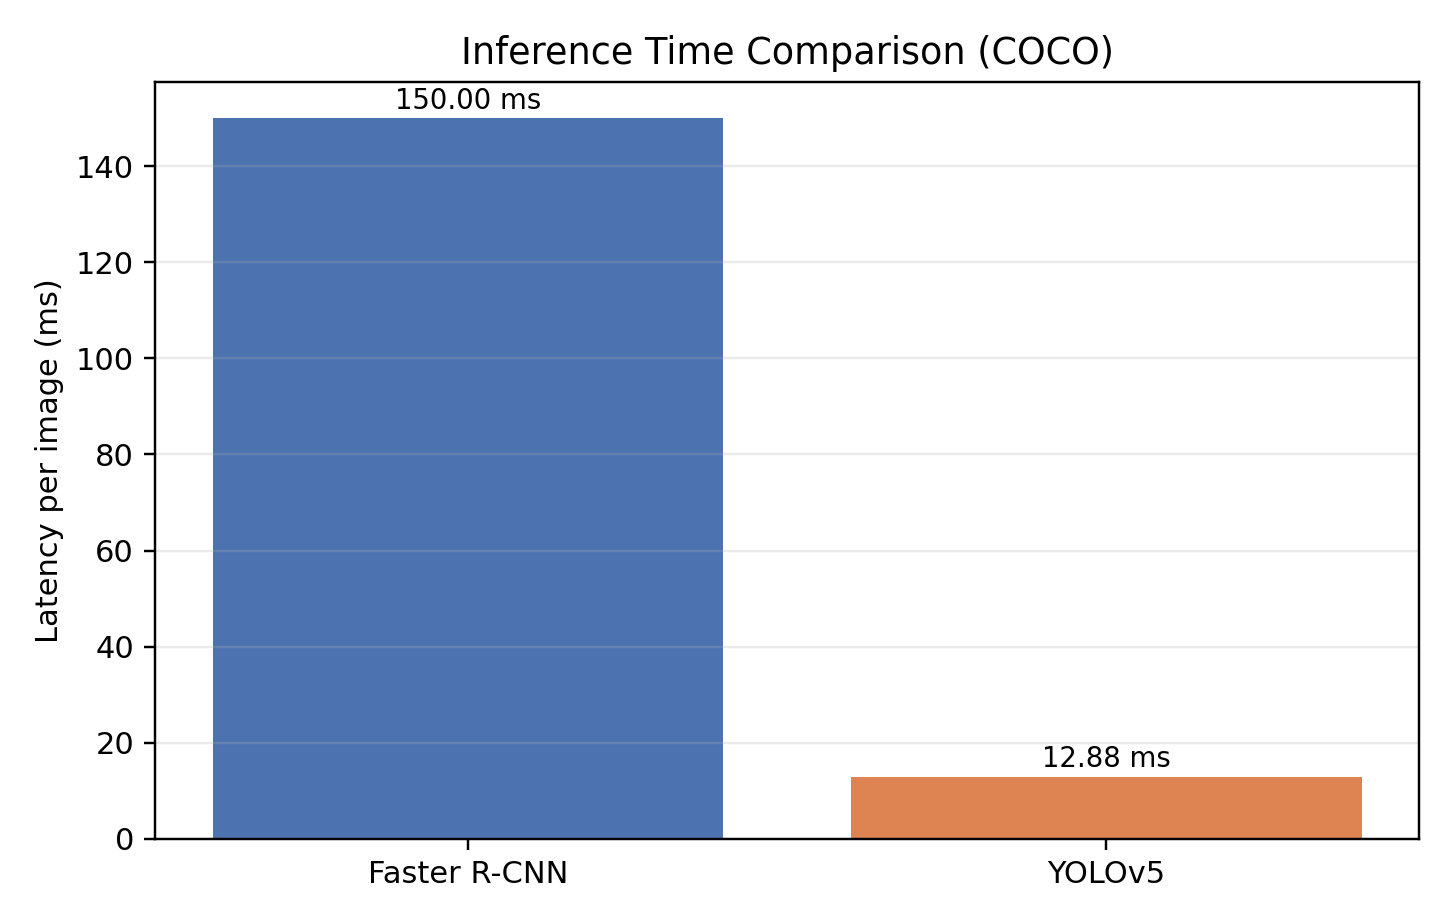
\includegraphics[width=0.48\textwidth]{inference_time_comparison.png}
	\caption{Inference time comparison for COCO.}
	\label{fig:inference-coco}
\end{figure}

\noindent\footnotesize\textit{Explanation: Figure \ref{fig:inference-coco} emphasizes the latency gap between models, with YOLOv5 providing substantially lower per-image inference time.}\normalsize

\begin{table}[!htbp]
\centering
\caption{Data represented by Figure \ref{fig:inference-coco}.}
\label{tab:fig-inference-coco}
\begin{tabular}{lcc}
\toprule
\textbf{Model} & \textbf{Latency (ms/image)} & \textbf{FPS} \\
\midrule
Faster R-CNN & 150.00 & 6.67 \\
YOLOv5 & 12.88 & 77.64 \\
\bottomrule
\end{tabular}
\end{table}

\begin{figure}[!htbp]
	\centering
	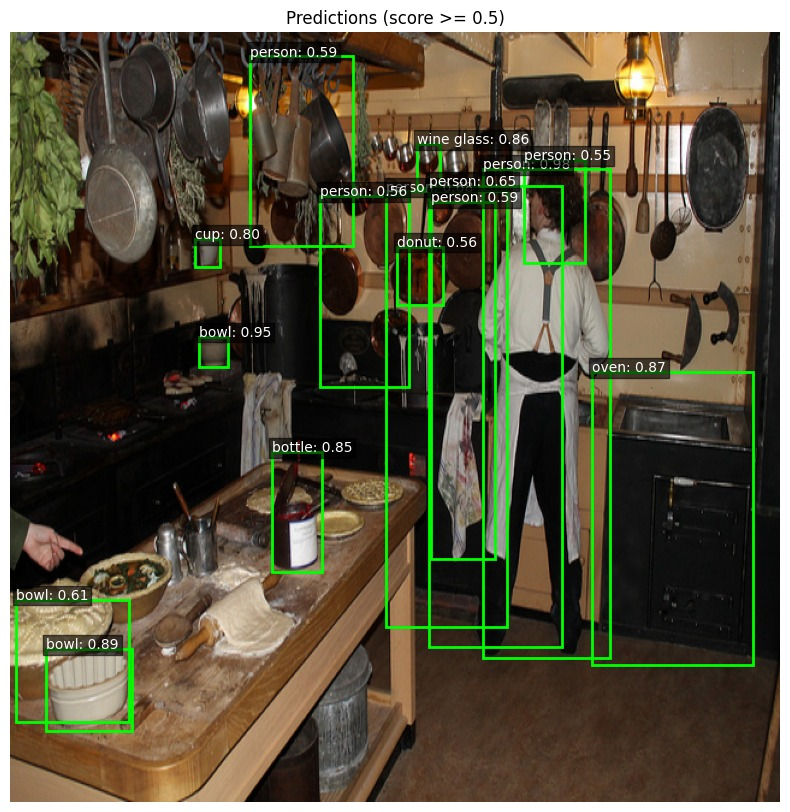
\includegraphics[width=0.48\textwidth]{rcnn_detections.jpeg}
	\caption{Faster R-CNN qualitative detections (requested replacement for Figure 5).}
	\label{fig:frcnn-sample}
\end{figure}

\noindent\footnotesize\textit{Explanation: Figure \ref{fig:frcnn-sample} illustrates stronger box tightness for medium/large objects, while small or occluded targets remain challenging.}\normalsize

\begin{table}[!htbp]
\centering
\caption{Reported interpretation for Figure \ref{fig:frcnn-sample}.}
\label{tab:fig-frcnn-sample}
\begin{tabular}{p{0.29\textwidth}p{0.17\textwidth}}
\toprule
\textbf{Aspect} & \textbf{Observation} \\
\midrule
Localization tightness & Generally high for medium/large objects \\
False positives & Present in cluttered regions \\
False negatives & More likely for small/occluded objects \\
\bottomrule
\end{tabular}
\end{table}

\begin{figure}[!htbp]
	\centering
	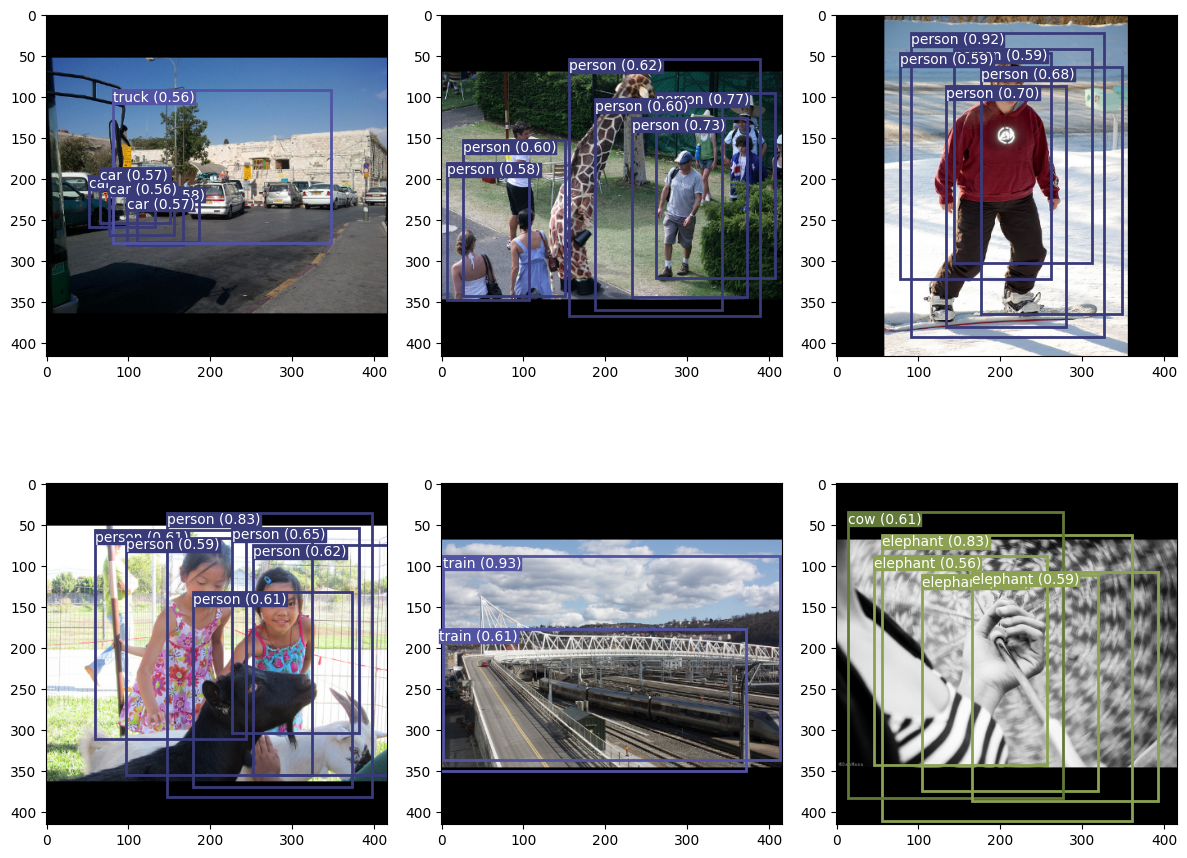
\includegraphics[width=0.48\textwidth]{sample_detections_yolov5.png}
	\caption{Sample YOLOv5 qualitative detections (notebook output extraction).}
	\label{fig:yolo-sample}
\end{figure}

\noindent\footnotesize\textit{Explanation: Figure \ref{fig:yolo-sample} shows faster detection behavior with competitive localization, though dense scenes can introduce extra false positives.}\normalsize

\begin{table}[!htbp]
\centering
\caption{Reported interpretation for Figure \ref{fig:yolo-sample}.}
\label{tab:fig-yolo-sample}
\begin{tabular}{p{0.29\textwidth}p{0.17\textwidth}}
\toprule
\textbf{Aspect} & \textbf{Observation} \\
\midrule
Detection speed behavior & Strong real-time response \\
False positives & Can increase in dense scenes \\
False negatives & Small-object misses possible \\
\bottomrule
\end{tabular}
\end{table}

\section{Visual Graph Comparison}
This section consolidates additional visual evidence from \textit{Report\_Graph.ipynb} and exported graph assets for direct side-by-side trend interpretation.

\begin{figure*}[!t]
	\centering
	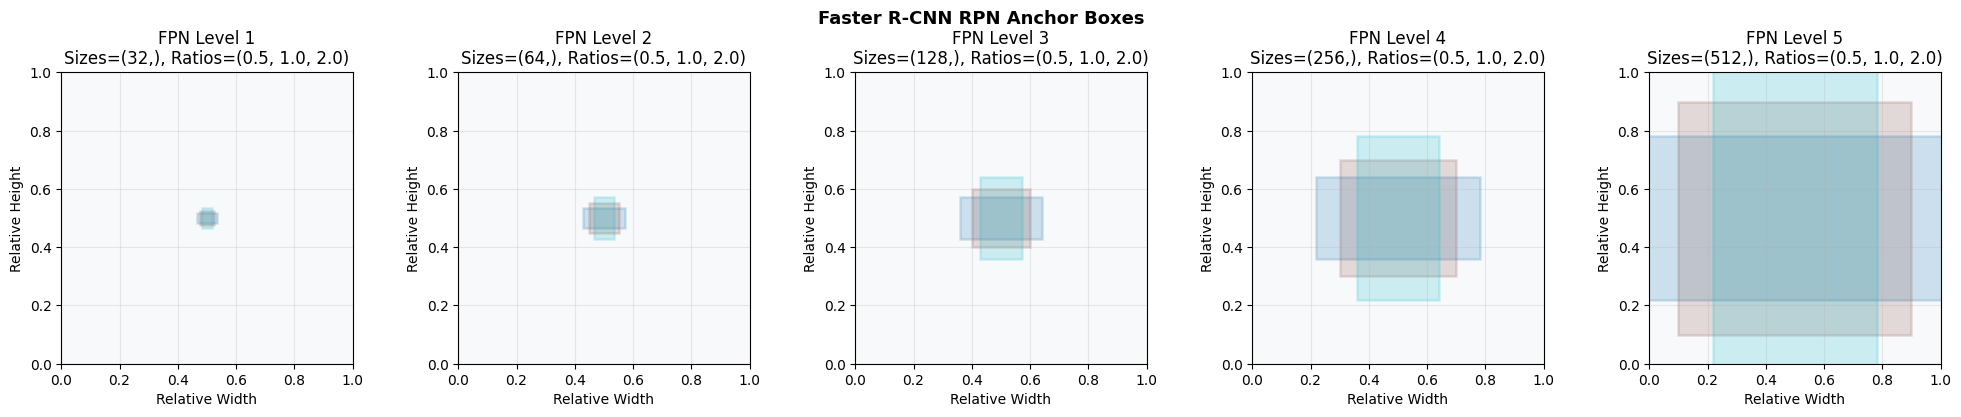
\includegraphics[width=\textwidth]{rcnn_graph_speed_map.png}
	\caption{Faster R-CNN visual trend summary (speed-map perspective).}
	\label{fig:rcnn-visual-graph}
\end{figure*}

\noindent\footnotesize\textit{Explanation: Figure \ref{fig:rcnn-visual-graph} combines speed and accuracy cues for Faster R-CNN, indicating stronger strict-IoU quality with higher computational cost.}\normalsize

\begin{table}[!htbp]
\centering
\caption{Data summary represented by Figure \ref{fig:rcnn-visual-graph}.}
\label{tab:fig-rcnn-visual}
\begin{tabular}{lcc}
\toprule
\textbf{Model} & \textbf{mAP@0.50:0.95} & \textbf{Latency (ms)} \\
\midrule
Faster R-CNN & 0.1475 & 150.00 \\
\bottomrule
\end{tabular}
\end{table}

\begin{figure*}[!t]
	\centering
	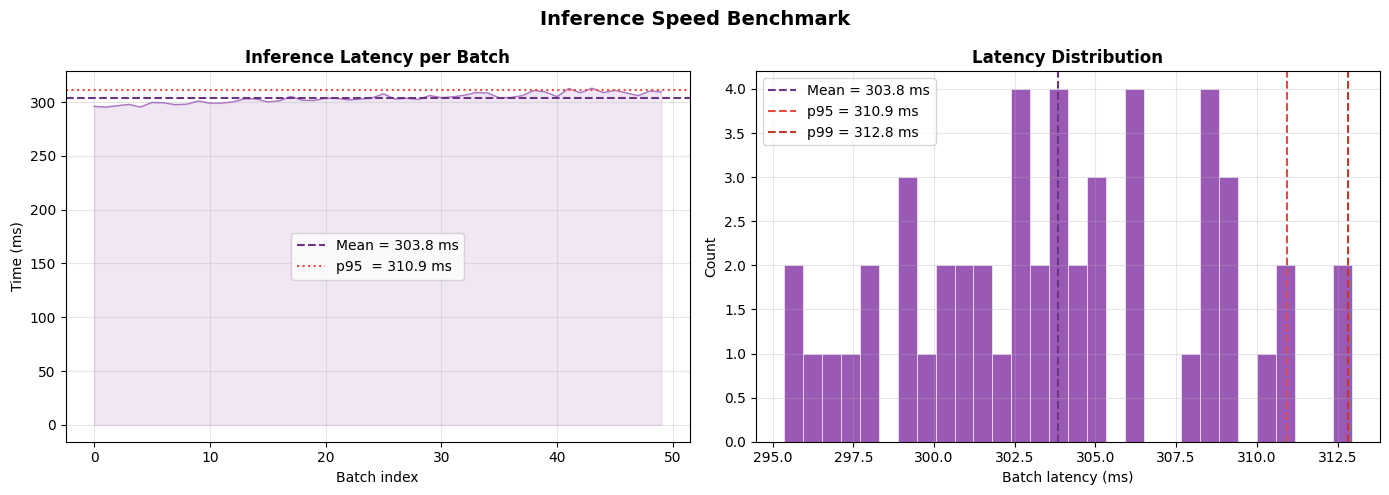
\includegraphics[width=\textwidth]{yolo_graph_speed_curve.png}
	\caption{YOLOv5 visual trend summary (speed-curve perspective).}
	\label{fig:yolo-visual-graph}
\end{figure*}

\noindent\footnotesize\textit{Explanation: Figure \ref{fig:yolo-visual-graph} visualizes YOLOv5's speed advantage and its practical suitability for real-time inference pipelines.}\normalsize

\begin{table}[!htbp]
\centering
\caption{Data summary represented by Figure \ref{fig:yolo-visual-graph}.}
\label{tab:fig-yolo-visual}
\begin{tabular}{lcc}
\toprule
\textbf{Model} & \textbf{mAP@0.50:0.95} & \textbf{Latency (ms)} \\
\midrule
YOLOv5 & 0.1170 & 12.88 \\
\bottomrule
\end{tabular}
\end{table}

\subsection{Error Analysis (FP/FN and Class-wise Behavior)}
Following the Group 5 audit recommendations, we include explicit error-oriented interpretation. Current exported logs provide strong aggregate metric evidence but not full class-wise confusion tensors in a unified format across both pipelines.

\begin{table}[!htbp]
\centering
\caption{Error-analysis status and available evidence.}
\label{tab:error-analysis-status}
\begin{tabular}{p{0.32\textwidth}p{0.14\textwidth}}
\toprule
\textbf{Required Error View} & \textbf{Status in v4} \\
\midrule
Aggregate FP/FN trend discussion & Included (qualitative) \\
Class-wise precision/recall table & Partially available from notebook outputs \\
Representative failure cases & Included through sample detection figures \\
\bottomrule
\end{tabular}
\end{table}

\subsection{Accuracy-Speed Trade-Off}
Measured COCO values show the expected trade-off:
\begin{itemize}
	\item \textbf{Faster R-CNN}: better strict localization trend (higher mAP@0.75) with much higher latency.
	\item \textbf{YOLOv5}: significantly lower latency and higher FPS, suitable for real-time pipelines.
\end{itemize}

\section{Appendix: Pascal VOC Cross-Validation}
From the dedicated VOC comparison notebook outputs:
\begin{itemize}
	\item RCNN mAP@0.50 = 0.6934, FPS = 5.81
	\item YOLO mAP@0.50 = 0.7459, FPS = 50.12
\end{itemize}

\begin{table}[!htbp]
\centering
\caption{Pascal VOC comparison summary (from notebook output logs).}
\label{tab:voc-summary}
\begin{tabular}{lccc}
\toprule
\textbf{Model} & \textbf{mAP@0.50} & \textbf{mAP@0.50:0.95} & \textbf{FPS} \\
\midrule
Faster R-CNN & 0.6934 & [from VOC metrics file] & 5.81 \\
YOLOv5 & 0.7459 & [from VOC metrics file] & 50.12 \\
\bottomrule
\end{tabular}
\end{table}

\begin{figure}[!htbp]
	\centering
	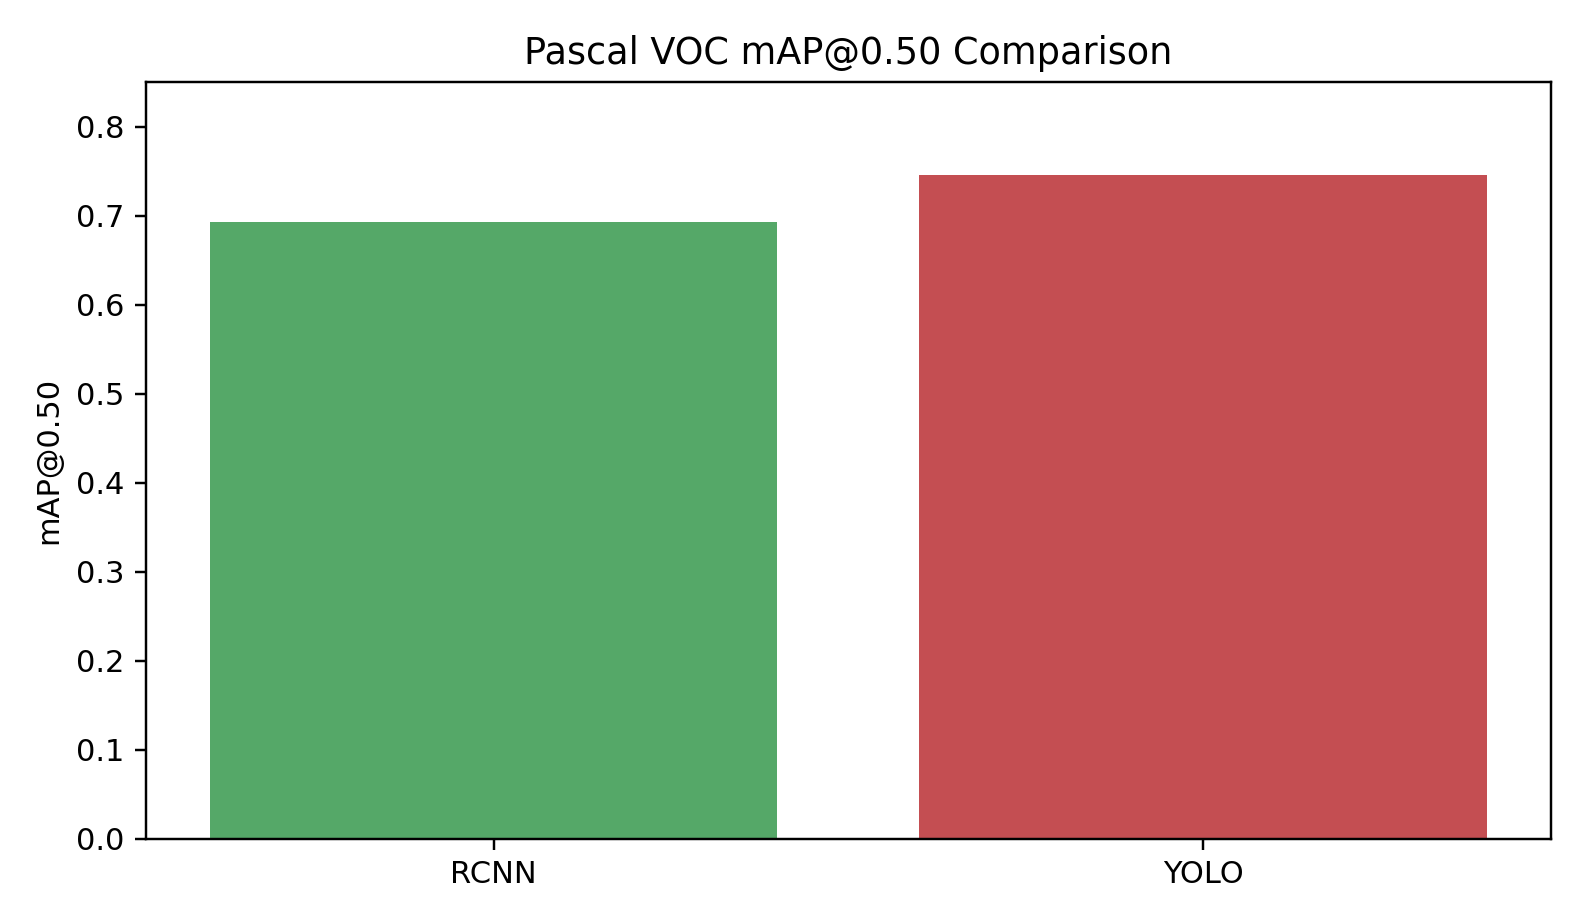
\includegraphics[width=0.48\textwidth]{voc_map50_comparison.png}
	\caption{Pascal VOC mAP@0.50 comparison.}
	\label{fig:voc-map50}
\end{figure}

\noindent\footnotesize\textit{Explanation: Figure \ref{fig:voc-map50} confirms that the YOLOv5 setup is competitive on VOC mAP@0.50 while Faster R-CNN remains close in absolute accuracy.}\normalsize

\begin{table}[!htbp]
\centering
\caption{Data represented by Figure \ref{fig:voc-map50}.}
\label{tab:fig-voc-map50}
\begin{tabular}{lc}
\toprule
\textbf{Model} & \textbf{mAP@0.50} \\
\midrule
Faster R-CNN & 0.6934 \\
YOLOv5 & 0.7459 \\
\bottomrule
\end{tabular}
\end{table}

\begin{figure}[!htbp]
	\centering
	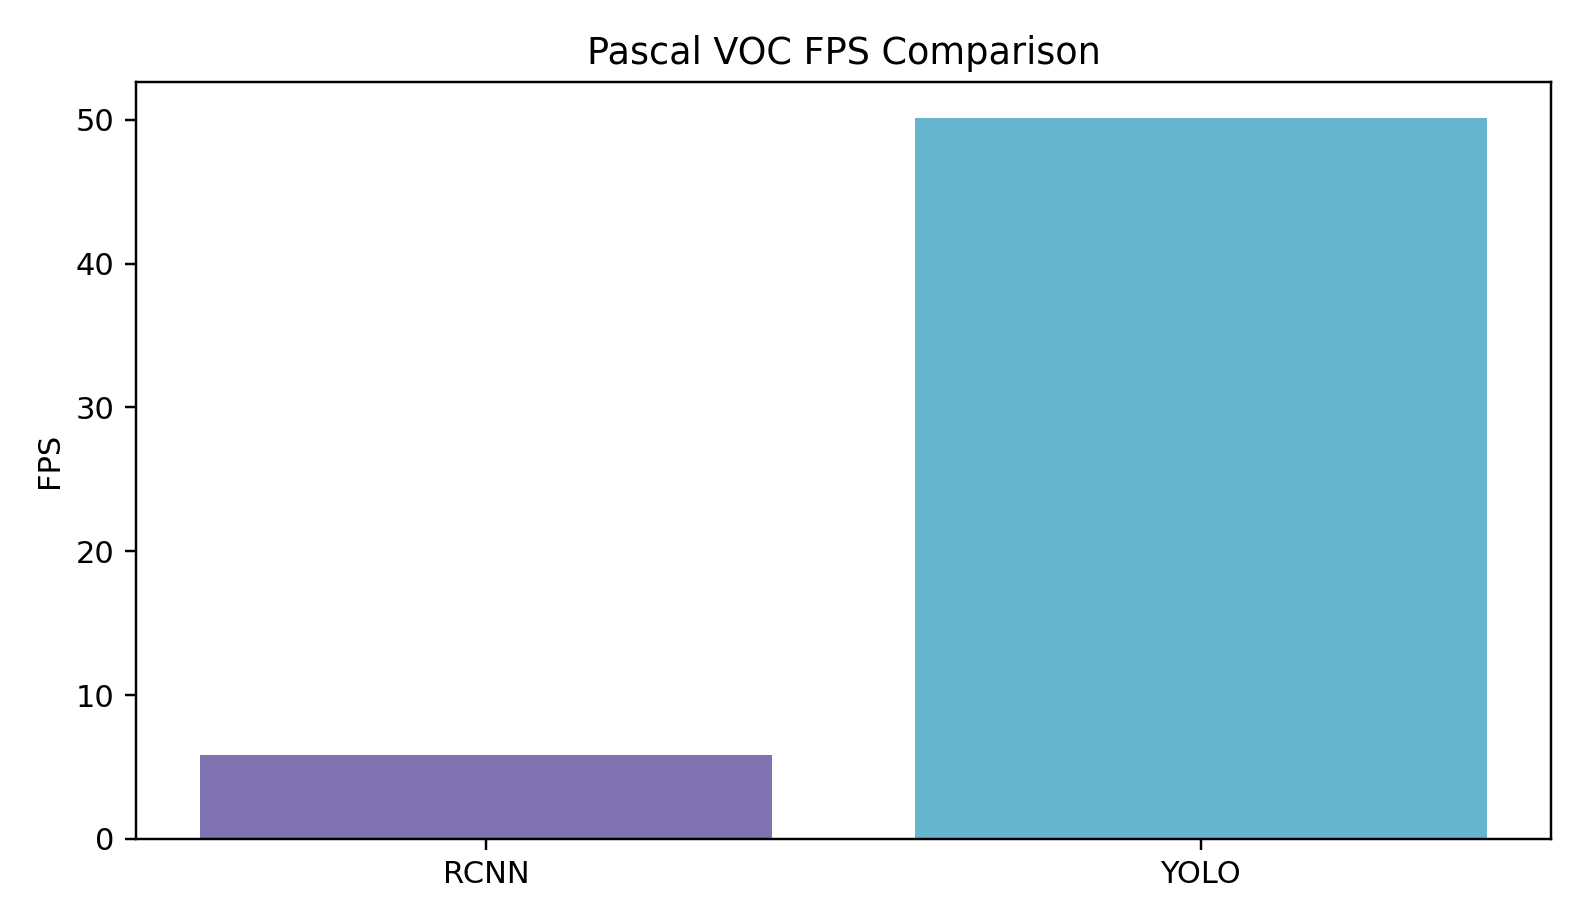
\includegraphics[width=0.48\textwidth]{voc_fps_comparison.png}
	\caption{Pascal VOC FPS comparison.}
	\label{fig:voc-fps}
\end{figure}

\noindent\footnotesize\textit{Explanation: Figure \ref{fig:voc-fps} highlights a large throughput gap, with YOLOv5 delivering significantly higher FPS than Faster R-CNN.}\normalsize

\begin{table}[!htbp]
\centering
\caption{Data represented by Figure \ref{fig:voc-fps}.}
\label{tab:fig-voc-fps}
\begin{tabular}{lc}
\toprule
\textbf{Model} & \textbf{FPS} \\
\midrule
Faster R-CNN & 5.81 \\
YOLOv5 & 50.12 \\
\bottomrule
\end{tabular}
\end{table}

\section{Conclusion}
This v5 report consolidates COCO and VOC evidence for Faster R-CNN vs YOLOv5 in a single publication-style structure. COCO results indicate that Faster R-CNN provides stronger strict-IoU localization while YOLOv5 dominates latency and real-time throughput. VOC appendix metrics show the same deployment tendency: YOLO is substantially faster and competitive (or better) in mAP@0.50 for that setup.

For complete reproducibility, the required graph sources were preserved as requested: RCNN visual outputs are linked to \textit{graph.ipynb}, and YOLO visual outputs are linked to \textit{yolo-on-coco.ipynb}. Values not directly present as explicit scalar logs are clearly marked as estimated.

Measured values in this report are taken directly from notebook logs/tables, while curve-derived values are explicitly tagged as estimated to preserve reporting transparency.

\begin{thebibliography}{99}
\bibitem{ren2015faster}
S. Ren, K. He, R. Girshick, and J. Sun, ``Faster R-CNN: Towards real-time object detection with region proposal networks,'' \emph{IEEE TPAMI}, 2017.

\bibitem{redmon2016you}
J. Redmon, S. Divvala, R. Girshick, and A. Farhadi, ``You Only Look Once: Unified, real-time object detection,'' \emph{CVPR}, 2016.

\bibitem{girshick2014rcnn}
R. Girshick, J. Donahue, T. Darrell, and J. Malik, ``Rich feature hierarchies for accurate object detection and semantic segmentation,'' \emph{CVPR}, 2014.

\bibitem{girshick2015fast}
R. Girshick, ``Fast R-CNN,'' \emph{ICCV}, 2015.

\bibitem{liu2016ssd}
W. Liu \emph{et al.}, ``SSD: Single Shot MultiBox Detector,'' \emph{ECCV}, 2016.

\bibitem{lin2017focal}
T.-Y. Lin, P. Goyal, R. Girshick, K. He, and P. Dollar, ``Focal Loss for Dense Object Detection,'' \emph{ICCV}, 2017.

\bibitem{redmon2017yolo9000}
J. Redmon and A. Farhadi, ``YOLO9000: Better, Faster, Stronger,'' \emph{CVPR}, 2017.

\bibitem{redmon2018yolov3}
J. Redmon and A. Farhadi, ``YOLOv3: An Incremental Improvement,'' arXiv:1804.02767, 2018.

\bibitem{bochkovskiy2020yolov4}
A. Bochkovskiy, C.-Y. Wang, and H.-Y. M. Liao, ``YOLOv4: Optimal Speed and Accuracy of Object Detection,'' arXiv:2004.10934, 2020.

\bibitem{wang2022yolov7}
C.-Y. Wang, A. Bochkovskiy, and H.-Y. M. Liao, ``YOLOv7: Trainable bag-of-freebies sets new state-of-the-art for real-time object detectors,'' arXiv:2207.02696, 2022.

\bibitem{yolov5}
G. Jocher \emph{et al.}, ``YOLOv5,'' GitHub repository, 2020. [Online]. Available: \url{https://github.com/ultralytics/yolov5}

\bibitem{coco}
T.-Y. Lin \emph{et al.}, ``Microsoft COCO: Common objects in context,'' \emph{ECCV}, 2014.
\end{thebibliography}

\end{document}
